\chapter{resultados preliminares}
\section{Desempenho Computacional}
Na Figura \ref{fig:clustera} s�o apresentados os valores de \textit{speed up} das
simula��es com diferentes n�meros de processadores. Como se pode perceber, foi 
poss�vel alcan�ar uma diminui��o no tempo de execu��o com as simula��es feitas em
paralelo, de forma que os valores de \textit{speed up} aumentam de forma linear,
aproximadamente. Na Figura \ref{fig:clusterb}, por sua vez, s�o apresentados os valores das
efici�ncias calculadas. Esses valores s�o
bem pr�ximos para 2, 4 e 8 processos, mas uma queda come�a a se tornar vis�vel em
16 processos, sugerindo que, a partir desse n�mero, a queda de efici�ncia se 
acentue.

\begin{figure}[ht!]
    \centering
    \subfloat[][]{
        \label{fig:clustera}
        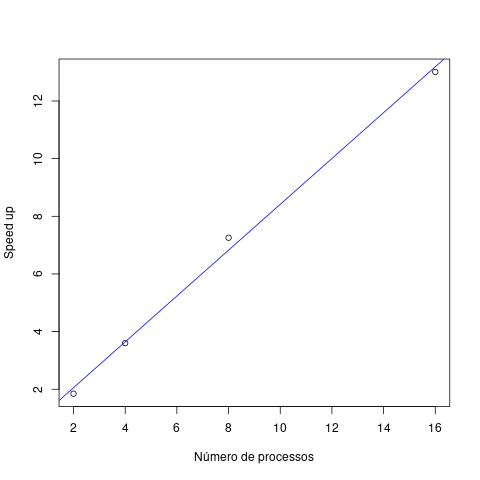
\includegraphics[scale=0.3]{linear}
    }
    ~ 
    \subfloat[][]{
        \label{fig:clusterb}
        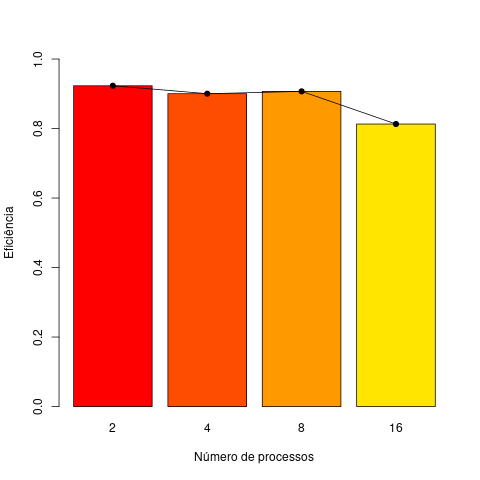
\includegraphics[scale=0.3]{efs}
    }
    \caption[Resultados de acelera��o e efici�ncia em fun��o do n�mero de processadores]{
        \subref{fig:clustera} Os c�rculos representam o \textit{speed up} obtido para cada
        n�mero de processador utilizado. A reta em azul mostra uma regress�o linear dos
        resultados. \subref{fig:clusterb} efici�ncia em fun��o do n�mero de processadores.
         }
\end{figure}

\section{Disparos dos Elementos Neuronais}
%como mostrado na Figura
%\subref*{fig:remotojavaspka},
%que foi gerada por meio de uma simula��o com 800 MNs do tipo S, 50 do tipo
%FR, 50 do tipo FF, 350 CRs e uma corrente de 40 nA injetada no soma de todos
%os MNs. Nesse gr�fico, os instantes de disparo dos MNs, representados por 
%�ndices, mostram MNs com �ndices menores disparando
%depois de outros com �ndices maiores. Como esses �ndices, na simula��o, est�o
%relacionados com o tamanho dos MNs, pode-se dizer que ocorreu um certa invers�o
%na ordem de recrutamento. 
%
%% TODO put figure in which FR and FF also fire
%\begin{figure}[ht!]
%    \centering
%    \subfloat[][]{
%        \label{fig:remotojavaspka}
%        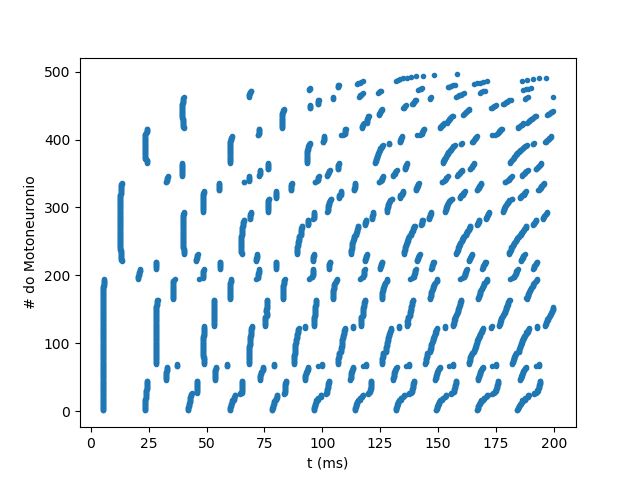
\includegraphics[scale=0.3]{remotojavaspk.png}
%    }
%    ~ 
%    \subfloat[][]{
%        \label{fig:remotojavaspkb}
%        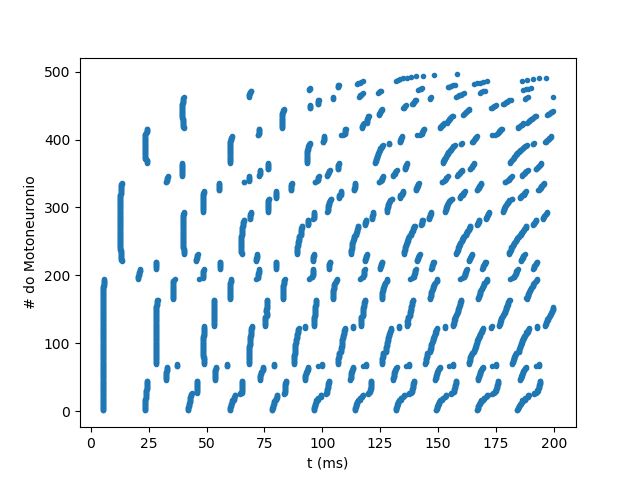
\includegraphics[scale=0.3]{remotojavaspk.png}
%    }
%    \caption[Momentos de disparo dos somas de todos os motoneur�nios simulados.]{
%             Momentos de disparo dos somas de todos os motoneur�nios simulados. O eixo 
%             das ordenadas representa o �ndice de cada motoneur�nio em ordem
%             crescente de tamanho.
%             \subref{fig:remotojavaspkb}.
%             \subref{fig:remotojavaspka}.
%         }
%\end{figure}
